\chapter{Resultados}

En este capítulo se presentan los datos obtenidos de la ejecución del proyecto bajo ciertas condiciones representativas, con la intención de validar la funcionalidad y también de encontrar los alcances y limites del mismo. Primero se estudiara el tiempo de respuesta de los algoritmos por separado, más tarde el rendimiento en la configuración mas simple, luego el sistema completo bajo condiciones de configuración varias y por ultimo el estudio de la mejora introducida por el uso de la cache.


\section{Caso Algoritmos únicamente}

Con la intención de obtener un gráfico que represente el rendimiento de los dos algoritmos implementados, se medirá el retardo de búsqueda en función de la posición en la tabla de enrutamiento, se realizaran las pruebas de manera independiente al modulo extracto de cabeceras. En el eje de las abscisas se expresa la ubicación en una tabla de 100 elementos y en las ordenadas se puede observar el tiempo de búsqueda en ciclos de reloj.

\begin{figure}[h]
  \centering
	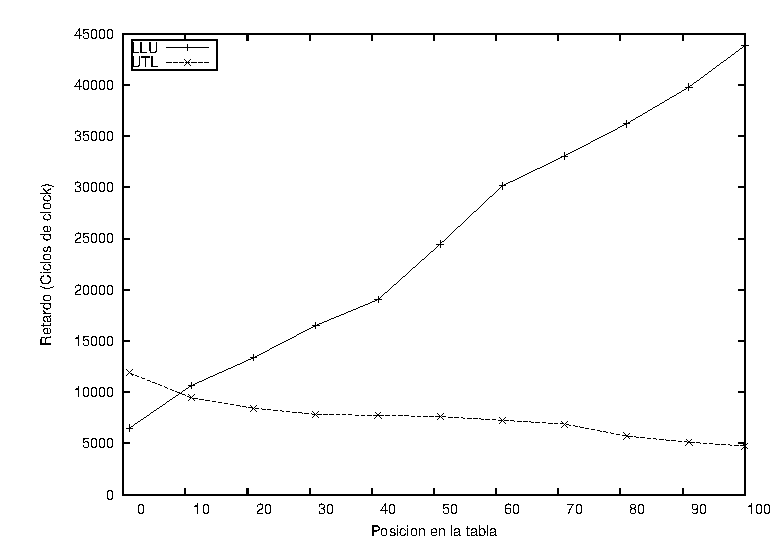
\includegraphics[width=0.8\textwidth]{5-resultados/graf/llu-utlsof.eps}
  \caption{Retardo de Búsqueda LLU vs UTL}
  \label{fig}
\end{figure}

\newpage
\section{Caso loopback}
\begin{figure}[h]
  \centering
	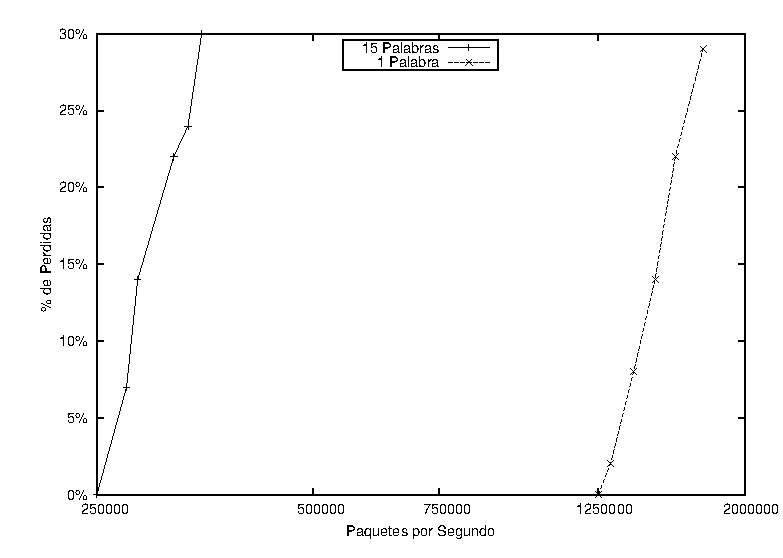
\includegraphics[width=0.70\textwidth]{5-resultados/graf/loop.eps}
  \caption{Caso Loopback para 1 y 15 palabras}
  \label{fig}
\end{figure}
Se estudia del caso loopback a los fines de encontrar los limites superiores de nuestro diseño. En este, el software solo se limita a recibir los datos e inmediatamente después confirma el procesamiento y envía los resultados de regreso al hardware. Se realizan las pruebas correspondientes para las dos versiones de Uplink.
En el eje de las abscisas es posibles ver la cantidad de paquetes por segundo, el origen corresponde a la mayor velocidad a la que es posible transmitir sin perdidas. En las Ordenadas se puede observar la cantidad de paquetes perdidos en valores porcentuales, para obtener esta métrica se proceso una cantidad constante de paquetes, 9000, y luego se contrasto este valor con un contador global que el Generador estampa en la ultima palabra de cada paquete. Así se calculo la cantidad paquetes perdidos, sobre la cantidad total de paquetes generados. Este mismo sistema es el usado en todos los gráficos posteriores.


\newpage
\section{Implementación Completa}

Se verificara el rendimiento del sistema implementado de manera completa. Se consideran seleccionaran tres puntos en las curvas que indican los tiempos de accesos del algoritmos, un punto mínimo que corresponde al menor tiempo de acceso, un punto promedio que ejercita 10 entradas equidistantes a lo largo de la tabla y un punto máximo que indica el peor tiempo de acceso posible para un Algoritmo dado. 

\subsubsection{Linear Lookup}
En la figura~\ref{figminllu} se puede observar que la diferencia en la cantidad de paquetes que pueden ser transmitidos sin errores en el mejor caso entre el modulo que envía una palabra al procesador y el que envía toda la cabecera, es considerable, mientras que a medida que aumenta la profundidad de búsqueda en la tabla estos valores convergen, como es posible ver en la figuras~\ref{figpromllu} y~\ref{figmaxllu}, lo que era esperable ya que para accesos muy lentos a la tabla el retardo introducido por el Hardware se vuelve despreciable.
\newpage
\begin{figure}[!h]
  \centering
	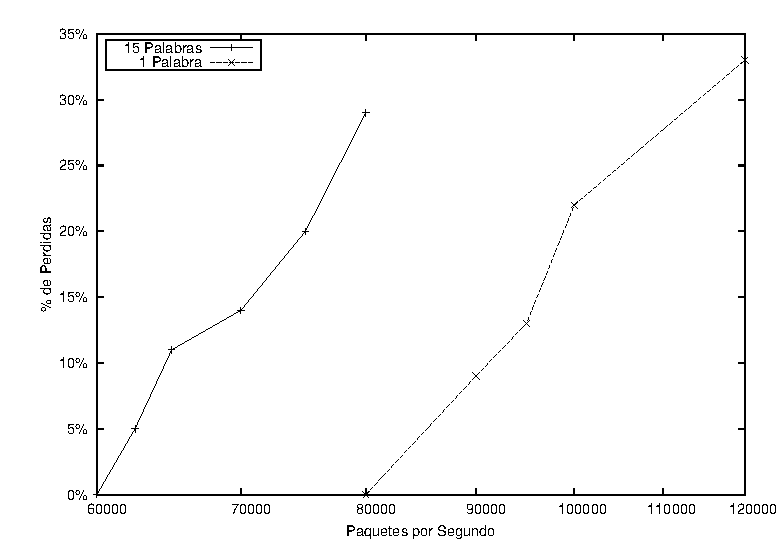
\includegraphics[width=0.7\textwidth]{5-resultados/graf/llumin.eps}
  \caption{Retardo mínimo LLU}
  \label{figminllu}
\end{figure}
\begin{figure}[!h]
  \centering
	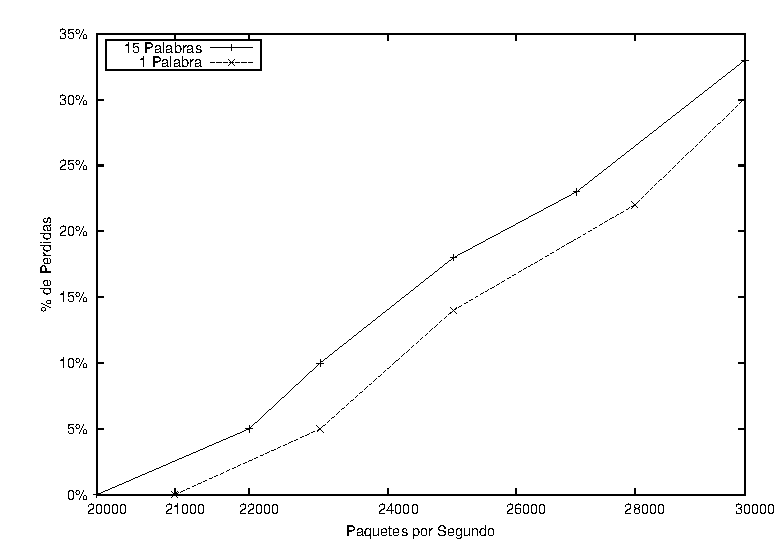
\includegraphics[width=0.7\textwidth]{5-resultados/graf/lluprom.eps}
  \caption{Retardo promedio LLU}
  \label{figpromllu}
\newpage
\end{figure}
\begin{figure}[!h]
  \centering
	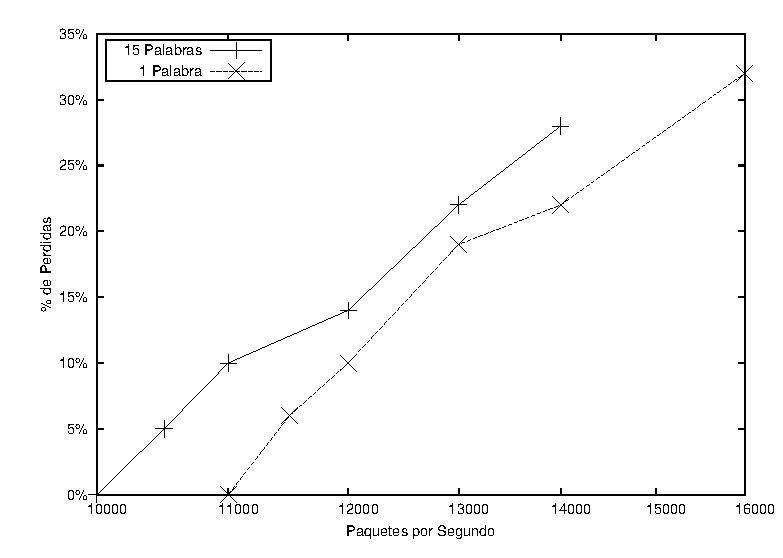
\includegraphics[width=0.7\textwidth]{5-resultados/graf/llumax.eps}
  \caption{Retardo máximo LLU}
  \label{figmaxllu}
\end{figure}



\newpage

\subsubsection{Unibit Trie Lookup}

En los gráficos que corresponden al Unibit Trie Lookup es posible observar que existe una menor diferencia entre la máxima cantidad de paquetes que pueden ser transmitidos sin error en cada uno de los 3 puntos elegidos. Así como también la diferencia entre enviar el paquete entero y solo la IP destino se reduce, lo que da la pauta de que cuando el tiempo de acceso es uniforme el impacto de la mejoras del Hardware tiende a ser menor.

\begin{figure}[!h]
  \centering
	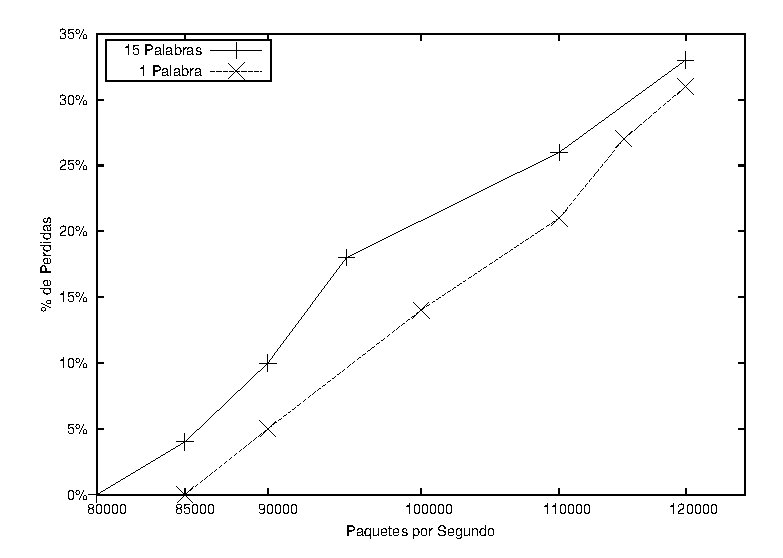
\includegraphics[width=0.7\textwidth]{5-resultados/graf/utlmin.eps}
  \caption{Retardo mínimo UTL}
  \label{fig}
\end{figure}
\begin{figure}[!h]
  \centering
	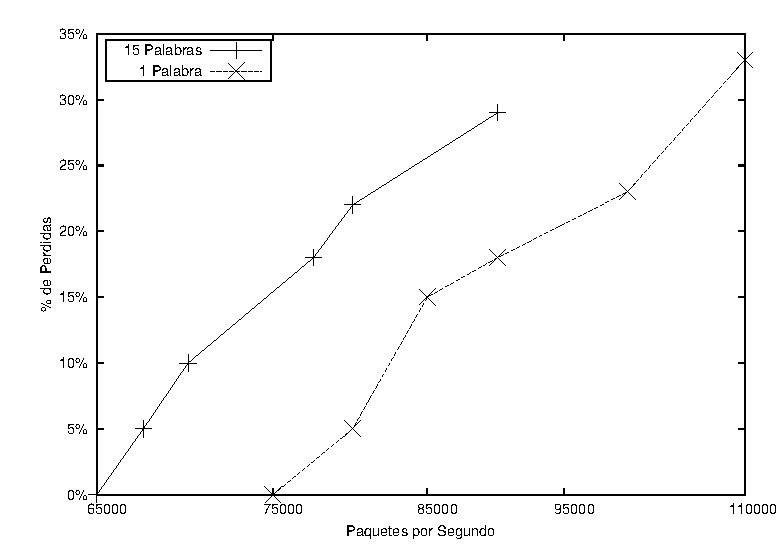
\includegraphics[width=0.7\textwidth]{5-resultados/graf/utlprom.eps}
  \caption{Retardo promedio UTL}
  \label{fig}
\end{figure}
\begin{figure}[!h]
  \centering
	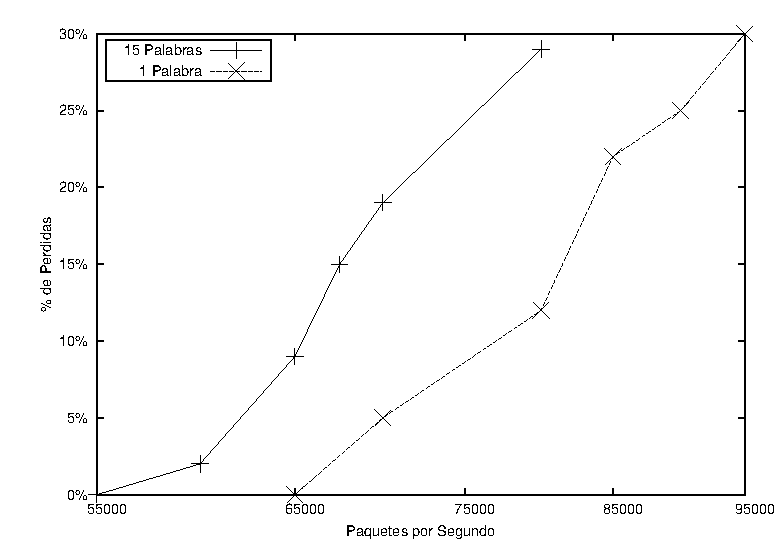
\includegraphics[width=0.7\textwidth]{5-resultados/graf/utlmax.eps}
  \caption{Retardo máximo UTL}
  \label{fig}
\end{figure}

(Falta la comparativa inter-algoritmos)


\newpage
\section{Cache}

(Falta Mejorar y agregar el grafico)
Se probara el funcionamiento del sistema incluyendo la cache implementada en software. Para ello, se efectuara una toma de datos en la cual se compararan 2 sucesiones: la primera de ella resultara en fallos al no estar presente ninguno de los valores.

Puede notarse que, en el caso de que la búsqueda termine en un fallo, se introduce un retardo adicional (si se compara con el escenario en el cual no existe la cache). Ello se debe a la búsqueda que se efectúa en la cache antes de hacerlo propiamente en la tabla de ruteo, tanto en la implementación linked-list como en la implementación unibit-trie.

